%*************************************************************************
% Chapter 1
%*************************************************************************


\chapter{Einleitung}
\label{ch:intro}
Das Thema Polystores ist bereits seit mehr als zehn Jahren Gegenstand aktiver Forschung. 
Dies ist relativ einfach damit zu begründen, dass die digitale Welt immer vielschichiger und komplexer wird.
Die Menge an zu verarbeitenden Daten steigt immer weiter. Wo es früher Ziel war, Datenbank Konzepte
zu entwerfen und zu implementieren, die möglichst sparsam mit der knappen Ressource Speicherplatz
umgehen, liegt heute der Fokus tendenziell auf Performance.
Empfehlungs-Systeme müssen in der Lage sein in Echtzeit oder sehr schnell auf Basis von Inputs
sinnvolle Vorschläge zum Beispiel im Kontext If a customer $\mathbf{C}$ bought item $\mathbf{A}$, then they also bought item $\mathbf{B}$ or item $\mathbf{C}$ or $\ldots$
:
\[
\forall c \in \mathcal{C} \quad \Bigl( \text{Bought}(c, A) \implies \bigl( \text{Bought}(c, B) \lor \text{Bought}(c, C) \lor \cdots \bigr) \Bigr)
\]
Ein solche Anfrage kann nur sinnvoll und performant beantwortet werden, 
wenn ein entsprechender Algorithmus sehr schnell Input von einer geeigneten
Datenbank erhält. Eine solche Datenbank, kann zum Beispiel eine Graph-Datenbank sein.
In zum Beispiel einem Web-Shop, wo ein solches Empfehlungs-System implementiert ist, entstehen
häufig auch typische Datenbank Transaktionen sog. Create, Read, Update, Delete Operationen (CRUD).
Solche Transaktionen können wiederum tendenziell besser über eine klassiche SQL Datenbank 
abgewickelt werden.
Eine solches System kann als ein Polystore bezeichnet werden, da es, um performant zu funktionieren,
mindestens zwei verschiedene Datenbank-Systeme bzw. Data-Stores benötigt.
Teilweise sind die Übergänge fließender als in dem oben genannten Beispiel des E-Commerce Systems 
mit einer Datenbank für die Empfehlungs-Engine und einer Datenbank für den transaktionsbasierten 
Teil des Systems.
So lassen sich zum Beispiel so genannte Datenströme genau so gut in eine zum Beispiel
dokumentenbasierte Datenbank abwickeln wie klassiche CRUD Operationen. Es wäre denkbar, dass beide
Teile eines fiktiven Systems über zum Beispiel eine MongoDB abgebildet werden.
Hier wäre es sinnvoll zu messen ob ein System welches aus zwei oder mehr verschiedenen Services besteht,
die sich einen Datastore bzw. ein Datenbank System teilen, bei einem sich dynamisch ändernden Workload,
eine Neuzzuteilung Service bzw. Dataset zu Datastore sinnvoll ist. Dies kann zum Beispiel sinnvoll sein,
wenn bestimmte Transaktionen oder Commits immer mehr Zeit in Anspruch nehmen, was sich wiederum
negativ auf die Benutzererfahrung bzw. die Performance des Systems auswirkt.
Grundsätzlich geht es also darum, dass in einem System S mindestens zwei verschiedene Services
S existieren,
die jeweils einem Datastore D zugeordnet sind und einen gewissen Workload W aufweisen. 
Ändert sich der Workload W bzw. werden bestimmte Grenzwerte Th überschritten, sollten die Services
bzw. der betroffene Service einem anderen, gegebenfalls besser geeigneten Datastore zugeordnet werden.
Dies sollte nur passieren, wenn der Service S in Verbindung mit dem neu zugewiesenen Datastore
einen verbesserten Workload aufweist.
Grundsätzlich kann der vorbezeichnete Sachverhalt wie folgt beschrieben werden:
\section*{Service Reassignment Based on Workload}

We define the following:

\begin{itemize}
    \item \textbf{Services:} 
    \[
    \mathcal{S} = \{ S_1, S_2, \ldots, S_n \} \quad (n \geq 2)
    \]
    \item \textbf{Datastores:} 
    \[
    \mathcal{D} = \{ D_1, D_2, \ldots, D_m \}.
    \]
    \item \textbf{Workload Function:} 
    \[
    W: \mathcal{S} \times \mathcal{D} \to \mathbb{R}_{\ge0},
    \]
    where \(W(S,D)\) measures the workload of service \(S\) when using datastore \(D\) (lower is better).
    \item \textbf{Thresholds:} Let \(Th \ge 0\) be the workload threshold, and let \(\epsilon > 0\) be a parameter defining a significant change in workload over time.
\end{itemize}

Let \(A: \mathcal{S} \to \mathcal{D}\) be the current assignment function, meaning that a service \(S\) is assigned to a datastore \(A(S)\).

For a given service \(S\), if either:
\[
\bigl|W(S, A(S))_t - W(S, A(S))_{t-1}\bigr| \ge \epsilon
\]
or
\[
W(S, A(S)) \ge Th,
\]
and there exists another datastore \(D' \in \mathcal{D}\) such that:
\[
W(S, D') < W(S, A(S)),
\]
then we reassign service \(S\) to \(D'\).

This rule can be written as:
\[
A'(S) =
\begin{cases}
D', & \text{if } \left( \bigl|W(S, A(S))_t - W(S, A(S))_{t-1}\bigr| \ge \epsilon \text{ or } W(S, A(S)) \ge Th \right) \\
    & \quad \text{and there exists } D' \in \mathcal{D} \text{ with } W(S, D') < W(S, A(S)); \\[1ex]
A(S), & \text{otherwise.}
\end{cases}
\]
Es gilt also permanent zu überprüfen wie ein System aus Datasets bzw. 
Services und Datastores aufgebaut sein sollte um die Anforderungen 
an dieses System optimal zu erfüllen. Genau diesem Thema widmet sich die forliegende Arbeit.
%
% Section: Motiva
%
\section{Motivation}
\label{sec:intro:motivation}
Es existieren bislang nur wenig bis gar keine polystoren Systeme die es über den Status Prototyp
geschafft haben. Das Projet was wohl am fortgeschrittensten ist ist Polyphenie DB.
Ein Erklärungsansatz für den mangelhafte Verbreitung von Polystore Systemen und oder deren 
produktiven Einsatz ist, dass die Implmentierung immer noch schwierig und aufwendig ist.

Ein anderer Erklärungsansatz ist, dass die Vorteile eines Polystores erst zum tragen 
kommen, wenn dieses in einem dynamischen Umfeld bzw. System zum Einsatz kommt. In einem dynamischen
Umfeld ändert sich der Workload und damit ist wie bereits beschrieben die initiale oder 
aktuelle Zuordnung von Datastores zu Datasets nicht mehr valide bzw. optimal.

Nun ist es schwer vorstellbar, dass in einem produktiven Betrieb permanent manuell Datasets
anderen Datenbanken und Datenbank Systemen zugeordnet werden. Ein solcher Eingriff ist komplex,
erfordert eine sorgfältige Vorbereitung und beansprucht in den meisten Fällen einen 
nicht unerheblichen Teil der Ressourcen (insbesondere Personal wie Datenbank Administratoren und 
Backend-Entwickler etc.). Des weiteren geht mit einer solchen Umstellung ein nicht
zu unterschätendes Risiko einher. Dieses Risiko kann durch bestimmte Verfahren wie das Testen 
der Umstellung in einer gekapselten Testumgebung, einer schrittweisen Umstellung etc. minimiert 
werden, dennoch sind Anpassungen am Datenmodell bzw. an der Persistenz-Schicht eines Systems immer heikel
und unterliegen häufig einem sehr statischen Setup.

Des Weiteren stellt sich immer die Frage wenn festgestellt wird, dass eine Zuordnung Datasets zu 
Datastores nicht mehr optimal ist, was die bessere Lösung wäre und wie sich der Workload durch eine 
Unmstellung potentiell verändern würde. Eine manuelle Überprüfung der Workloads ist zwar denkbar aber schwer
mit dem Alltag von Entwicklungs-Teams vereinbar. 
Wenn man feststellt, dass die Performance aber auch andere parameter wie Verfügbarkeit, also letztendlich
Service Level Agreements (SLA) nicht mehr den Anforderungen entsprechen, stellt sich die Frage, wie 
das System umgestellt werden sollte oder umgestellt werden kann um die Anforderungen wieder 
zu erfüllen.

Die weiterführende Vision bzw. Motivation dieser Arbeit ist, eine Polystore System welches auf Basis
von Workloads, Applikationsparametern und SLA automatisch eine initial Zuordnung von Datasets zu Datastores vornimmt
und dieses Setup kontinuierlich und automatisiert überwacht und im Fall von Abweichungen 
sich selbst optimiert. Ein solches System wäre gerade für komplexe Anwendungen mit heterogenen Anforderungen
an die entsprechenden Datastores ein Mehrwert und trägt der Erkenntnis Rechnung 
das im Bereich Datastores und Datenbank eine One Fits All Lösung nicht bzw. bislang niht existiert.
So entsteht für den Benutzer ein optimiertes Nutzererlebnis und das Entwicklungs-Team kann sich voll 
auf die Implmentierung von User Interfaces und Business Logik fokussieren.

%
% Section: Ziele
%
\section{Ziele der Arbeit}
\label{sec:intro:goal}
Die Ziele der Arbeit sind wie folgt: \\

1. Einen theoretischen Überblick zu lieferen, wie ein dynamisches polystore basiertes System beschaffen 
sein muss bzw. beschaffen sein sollte, damit dieses in produktiven Umgebungen eingesetzt werden  kann.
\\

2. Konkret zu beschreiben welche Schritte ein dynamisches polystore basiertes System immer wieder durchlaufen 
muss um sich selbst aktuell zu halten und ein möglichst optimalen fit zwischen Datasets und Datastores
zu generieren.
\\
3. Einen Prototyp zu implementieren, der auf Basis von definierten Inputs eine intiale Zuordnung von 
Datasets zu Datastores herstellt. 

4. Auf Basis des Prototyp aus 3. einen Algorithmus zu implementieren, der den Workload von Datastores
analysiert und dynamisch neue Zuordnungsvorschläge generiert, wenn sich der Workload verändert.

5. Theoretisch zu beschreiben welche Schritte unternommen werden müssen, um eine dynamisch errechnete
neue Zuordnung von Datasets zu Datastores zu exekutieren.

% Section:  der Arbeit
%
\section{Gliederung}
\label{sec:intro:structure}

Die Arbeit ist wie folgt gegliedert:

Nach der Einleitung werden in Chapter2 TODO Terminologische Grundlagen die für das Verständnis
der Arbeit wichtig sind erörtert.

In Chapter3 TODO beginnt der Hauptteil der Arbeit, der sich mit den Zielen 1. und 2. aus Chapter TODO 
beschäftigt. In diesem Kapitel soll vor allem ein Überblick vermittelt werden, wie 
dynamisch polystore basiertes System funktionieren kann und welche Kernelemente und Schnittstellen 
dieses enthalten muss.

Chapter4 beschäftigt sich mit der Implmentierung der Prototypen in Verbindung mit den Zielen 4 und 5 TODO.
Es soll Konkret beschrieben werden wie der Prototyp aufgebaut ist bzw. der Algorithmus zur 
dynamischen Neuzuteilung funktioniert. Zusätzlich werden die Ergebnisse aus dem Testbetrieb beschrieben
und gegebenfalls sinnvolle Ergänzungen und oder Einschränkungen bezogen auf den praktischen Einsatz 
dokumentiert.

Chapter5 beschreibt die konkreten Schritte zur Umsetzung einer dynamischen Neuzuteilung von Datasets
zu Datastores. Wie können Schnittstellen aussehen oder müssen diese beschaffen sein um Datasets 
einen neuem Datastore zuzuweisen? Welche Rolle spielen Konzepte wie Objekt Relationale Mapper (ORM)?
Welche konkreten Arbeitsschritte müssen durchlaufen wie durchlaufen werden um die neue Zuordnung
so umzusetzen, dass die zu Grunde liegende Anwendung oder das zu Grunde liegende System weiter 
arbeitsfähig ist? Welche Service Level Agreements müssen wie eingehalten werden und was bedeuten
zum Beispiel Anforderungen wie eine Zero Downtime für ein solches System?

In Chapter 6 werden die Ergebnisse aus dem Hauptteil (TODO Chapter3 bis Chapter5) zusammengefasst.
Zusätzlich soll ein Ausblick gegeben und Empfehlungen gegeben werden, wie das Thema dynamische 
Polystores weiter entwickelt werden können.
Die Arbeit endet mit einem Fazit bezogen auf die zusammengefassten Ergebnisse und den Ausblick.


%*************************************************************************
% Chapter 2
%*************************************************************************


\chapter{Terminologische Grundlagen}
Nach der Einleitung sollen nun in diesem Kapitel wichtige Terminologische Grundlagen geklärt werden,
um ein einheitliches Verständnis zu generieren.

Dataset

A dataset is a structured collection of related data that is organized for efficient storage, retrieval, and analysis. 
In the context of datasets and datastores, it typically refers to:

Organization: Data arranged in a systematic format (e.g., tables, files, or arrays) that can be easily queried or processed.\newline
\\
Purpose: Aimed at supporting tasks like analysis, reporting, or machine learning model training.\newline
\\
Metadata: Often accompanied by metadata that describes the structure, source, and meaning of the data, enhancing its usability. \newline
\\
Storage: May be stored in various datastores such as databases, file systems, or cloud storage services, ensuring accessibility and scalability.

Datastore

A datastore is a system or repsitory designed for the storage, management, and retrieval of data, including datasets and other data objects. In the context of datasets and datastores:

Storage Mechanism: A datastore provides the underlying nfrastructure to physically or logically store data. This can be implemented as a database, file system, data warehouse, or cloud storage service\newline
\\
    Management and Retrieval: It offers methods for efficiently accessing, querying, and updating the stored data. This might involve indexing, transaction management, or specialized query languages.
\\
    Data Integrity and Security: Datastores often include mechanisms for ensuring data accuracy, consistency, and protection against unauthorized access.
\\
    Scalability: They are built t handle varying amounts of data, supporting growth and high performance as data volume increases.
\\

Datasets and Datastores\\

In summary, while a dataset is the structured collection of data used for analysis or processing, 
a datastore is the system that houses and manages these datasets, ensuring that data is organized, accessible, and secure.

Nach dem die grundsätzlichen Begriffe Datasets und Datastores geklärt sind, werden die beiden Begriffe Mulltistore und 
Polystore definiert und voneinander abgegrenzt. Beide Konzepte honorieren, dass eine One Size fits all Lösung für 
verschiedenartige Datassets nicht existiert und pro Dataset er jeweils best passende Datastore genutzt werden sollte.


Multistore

Ein Multistore besteht aus einer einzigen öffentlichen Schnittstelle und übersetzt die Anfragen an diese 
Schnittstelle zu Query Interface der verschiedenen und verschiedenartigen Datastores Dij wobei i den jeweiligen Datastore
identifiziert und j den Typ des Datastores abbildet:

\begin{figure}[htbp]
    \centering
    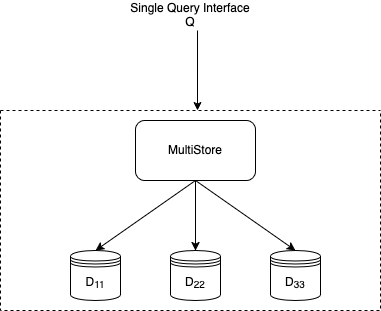
\includegraphics[width=0.60\textwidth]{gfx/examples/master_thesis-multistore.png}
    \caption{Concept of a Multistore}
    \label{fig:multistore}
\end{figure} 


Polystore
Ein Polystore wiederum bietet verschiedene öffentliche Schnittstellen Q1,...,QN und leitet die Anfragen an die entsprechenden 
Datastores 1,...,N weiter.

\begin{figure}[htbp]
    \centering
    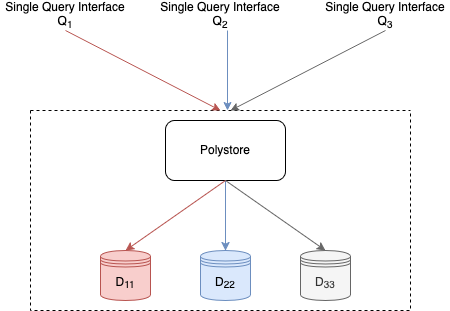
\includegraphics[width=0.60\textwidth]{gfx/examples/master_thesis-polystore.png}
    \caption{Concept of a Multistore}
    \label{fig:multistore}
\end{figure} 

%*************************************************************************
% Chapter 3
%*************************************************************************

\chapter{Initial Zuordnung von Datasets zu Datastores}


%*************************************************************************
% Chapter 4
%*************************************************************************

\chapter{Dynamische Allokation und Re-Allokation von Datasets zu Datastores}


%*************************************************************************
% Chapter 5
%*************************************************************************

\chapter{Datenmodell und Datenbankseitige Umsetzung von Datastore Re-Allokationen}

%*************************************************************************
% Chapter 6
%*************************************************************************

\chapter{Schlussbetrachtung}